\documentclass[xcolor=pdftex,dvipsnames,table,aspectratio=169]{beamer}
%\documentclass[xcolor=pdftex,dvipsnames,table,handout,aspectratio=169]{beamer}

%\setbeameroption{show notes}

\usepackage{bm,graphicx,multirow,amsmath,tikz} %fancybox,
\usepackage{color}%,textpos}
\usepackage[round]{natbib}
\usepackage[normalem]{ulem}
\usepackage{hyperref}
\usepackage{lastpage}
\usepackage{array}
\usepackage{color}
\usepackage{framed}
\usepackage{hyperref}

% Define Western colours
\definecolor{western}{rgb}{.306,.152,.524}
\definecolor{westerngray}{rgb}{.512,.508,.524}

%% Define BEAMER colours
\setbeamercolor{frametitle}{bg=western,fg=white}
\setbeamercolor{framesubtitle}{bg=western,fg=black}
\setbeamercolor{title}{fg=white,bg=western}
\setbeamercolor{author}{fg=white,bg=western}
\setbeamercolor{institute}{fg=white,bg=western}
\setbeamercolor{date}{fg=white,bg=western}

%% Set BEAMER fonts
\setbeamerfont{title}{shape=\bf}
\setbeamerfont{frametitle}{shape=\sc,size=\Large}
\setbeamerfont{framesubtitle}{shape=\sc,size=\Large}
\setbeamerfont{footline}{shape=\sc}

%% Define BEAMER toc
\setbeamercolor{section in toc}{fg=western}
\setbeamercolor{subsection in toc}{fg=westerngray}
\setbeamertemplate{sections/subsections in toc}[ball]

%% Define BEAMER background
\setbeamercolor{background canvas}{bg=white}

%% Define BEAMER footer
\setbeamertemplate{navigation symbols}{}
\setbeamercolor{footline}{fg=white,bg=western}
\setbeamertemplate{footline}{%
  \begin{beamercolorbox}[wd=\paperwidth]{footline}
    \vskip5pt

    \raisebox{.05in}{
      \scriptsize{\bf \insertshorttitle}
    }
    \hfill
    \raisebox{.05in}{
      \scriptsize{\bf \insertframenumber/\inserttotalframenumber} 
    }
    \hspace{5pt}

    \vskip5pt
  \end{beamercolorbox}
}

%% Define BLOCK environment
\setbeamercolor{block title}{fg=western}
\setbeamerfont{block title}{series=\bfseries}

%% Define ENUMERATE and ITEMIZE environements
\setbeamertemplate{itemize item}[ball]
\setbeamertemplate{enumerate item}[ball]
\setbeamercolor{item projected}{bg=western}

%% Define BEAMER toc
\setbeamercolor{sections/subsections in toc}{fg=blue!75}
\setbeamertemplate{sections/subsections in toc}[ball]

% %% Define SECTION openings
% \AtBeginSection[]{
%   \begin{frame}{\insertshorttitle}
%     \tableofcontents[currentsection,subsectionstyle=hide/hide/hide]
    
%   \end{frame}
% }

%% Define BEAMER frametitle
\addtobeamertemplate{frametitle}{
   \let\insertframetitle\insertsectionhead}{}
\addtobeamertemplate{frametitle}{
   \let\insertframesubtitle\insertsubsectionhead}{}


\makeatletter
  \CheckCommand*\beamer@checkframetitle{\@ifnextchar\bgroup\beamer@inlineframetitle{}}
  \renewcommand*\beamer@checkframetitle{\global\let\beamer@frametitle\relax\@ifnextchar\bgroup\beamer@inlineframetitle{}}
\makeatother

% Define counters for example and exercise
\newcounter{example}
\newcounter{exercise}

% Define example and exercise commands
\renewcommand{\example}
{\stepcounter{example}Example \lecturenum.\arabic{example}}
\newcommand{\examplectd}
{Example \lecturenum.\arabic{example}\ ctd}
\newcommand{\exercise}
{\stepcounter{exercise}Exercise \lecturenum.\arabic{exercise}}
\newcommand{\exercisectd}
{Exercise \lecturenum.\arabic{exercise}\ ctd}

\newcommand{\lecturenum}{22}

\title[SS2857]{Probability and Statistics I}
\subtitle{\lecturenum.~Conditional Distributions}

\date{}

%% Add logo
%% \titlegraphic{\includegraphics[height=2cm]{../uwo_logo_reversed}}

%% Initialize R


\begin{document}

{
\setbeamertemplate{footline}{}
\setbeamercolor{background canvas}{bg=western}

\begin{frame}
  \addtocounter{framenumber}{-1}

  \maketitle
\end{frame}
}

\begin{frame}
  \frametitle{\invisible{Hello}}
  
  \begin{center}
    \Large{\textbf{5.3 Conditional Distributions}}

    \bigskip

    \Large{Discrete Random Variables}
  \end{center}
  
\end{frame}

\section{Discrete Random Variables}
\label{sec:two-discrete-random}



\begin{frame}

  \begin{block}{Conditional Probability Mass Function}
    
    Let $X$ and $Y$ be two discrete random variables with joint pmf $p(x,y)$. The conditional pmf of $Y$ given $X=x$ ($Y|X=x$) for any value $x$ such that $p_X(x)>0$ is
    \[
      p_{Y|X}(y|x)=\frac{p(x,y)}{p_X(x)}.
    \]
  \end{block}
\end{frame}

\begin{frame}

  \begin{block}{Conditional Mean and Variance}
    
    The expected value and variance of $Y|X=x$ are
    \[
      \mu_{Y|X=x}=E(Y|X=x)=\sum_{y\in D_y} yp_{Y|X}(y|x)
    \]
    and
    \begin{align*}
      \sigma^2_{Y|X=x}=V(Y|X=x)&=E[(Y-E(Y|X=x))^2|X=x]\\
                   &=E[Y^2|X=x]-E[Y|X=x]^2.
    \end{align*}
  \end{block}
\end{frame}

\begin{frame}

  \begin{block}{Independence}
    
    Two discrete random variables $X$ and $Y$ are said to be independent if
    \[
      p(x,y)=p(x)p(y)
    \]
    for every $x \in \mathcal{X}$ and $y \in \mathcal{Y}$. 
    
    \bigskip
    
    Alternatively, $X$ and $Y$ are independent if
    $$
    p_{Y|X}(y|x)=p_Y(y) \Leftrightarrow p_{X|Y}(x|y)=p_X(x).
    $$
  \end{block}
\end{frame}

\begin{frame}
  \begin{block}{\example: Berkeley Admissions Data Revisited}
    In Example 20.1 we approximated the joint and marginal pmfs of gender ($X$) and department ($Y$) of an applicant to as:
    \begin{center}
      \begin{tabular}{lrr|r}
        \hline
        Major & Men & Women & $p_Y(y)$\\ 
        \hline
        A & 0.182 & 0.024 & .206\\ 
        B & 0.124 & 0.006 & .130\\ 
        C & 0.072 & 0.131 & .203\\ 
        D & 0.092 & 0.083 & .175\\ 
        E & 0.042 & 0.087 & .129\\ 
        F & 0.082 & 0.075 & .158\\ 
        \hline
        $p_X(x)$ & .595 & .405
      \end{tabular}
    \end{center}
  \end{block}
  
\end{frame}

\begin{frame}
  \begin{block}{\examplectd}
    
    \begin{enumerate}[a)]
    \item Find the conditional pmf of $X$
      \begin{enumerate}[i.]
      \item given $Y=1$ 
      \item given $Y=2$.
      \end{enumerate}
    \item Compute the conditional mean and variance of $X$
      \begin{enumerate}[i.]
      \item given $Y=1$
      \item given $Y=2$.
      \end{enumerate}        
    \item Comment on the results.
    \end{enumerate}
  \end{block}
\end{frame}


\begin{frame}
  \frametitle{\invisible{Hello}}
  
  \begin{center}
    \Large{\textbf{5.3 Conditional Distributions}}

    \bigskip

    \Large{Continuous Random Variables}
  \end{center}
  
\end{frame}

\section{Continuous Random Variables}

\begin{frame}

  \begin{block}{Conditional Probability Density Function}
    Let $X$ and $Y$ be two discrete random variables with joint pdf $f(x,y)$. The conditional pmf of $Y$ given $X=x$ ($Y|X=x$) for any value $x$ such that $f_X(x)>0$ is
    \[
      f_{Y|X}(y|x)=\frac{f(x,y)}{f_X(x)}.
    \]
  \end{block}
\end{frame}

\begin{frame}

  \begin{block}{Conditional Mean and Variance}
    The expected value and variance of $Y|X=x$ are
    \[
      \mu_{Y|X=x}=E(Y|X=x)=\int_{-\infty}^\infty y f_{Y|X}(y|x) ~dy
    \]
    and
    \begin{align*}
      \sigma^2_{Y|X=x}=V(Y|X=x)
                 &=E[(Y-E(Y|X=x))^2|X=x]\\
                 &=E[Y^2|X=x]-E[Y|X=x]^2.
    \end{align*}
  \end{block}
\end{frame}

\begin{frame}
  \begin{block}{Independence}
    Two continuous random variables $X$ and $Y$ are said to be independent if
    \[
      f(x,y)=f_X(x)f_Y(y)
    \]
    for every $(x,y)\in \mathbb R^2$. 
    
    \bigskip
    
    Alternatively, $X$ and $Y$ are independent if
    $$
    f_{Y|X}(y|x)=f_Y(y) \Leftrightarrow f_{X|Y}(x|y)=f_X(x).
    $$
  \end{block}
\end{frame}

\begin{frame}
  \begin{block}{\example}
    In Example 20.2 we considered the random variables $X$ and $Y$ with joint pdf
    \[
      f(x,y)=
      \left\{
        \begin{array}{ll}
          \frac{9}{16}(1-x^2)(1-y^2) & -1 < x,y < 1\\
          0 & \mbox{otherwise}
        \end{array}
      \right.
    \]

    \begin{enumerate}[a)]
    \item Compute the conditional pdf of $Y$ given $X=0$ and $X=.5$. 
    \item Compute the conditional mean of $Y$ given $X=0$ and $X=.5$.
    \item Comment on the results.
    \end{enumerate}
  \end{block}
\end{frame}

\begin{frame}
  \frametitle{\invisible{Hello}}
  
  \begin{center}
    \Large{\textbf{5.3 Conditional Distributions}}

    \bigskip

    \Large{Bivariate Normal}
  \end{center}
  
\end{frame}

\section{Bivariate Normal Distribution}

\begin{frame}
  \begin{block}{Bivariate Normal}
    We say that $X$ and $Y$ have a bivariate normal distribution with means $\mu_1$ and $\mu_2$, variances $\sigma^2_1$ and $\sigma^2_2$, and correlation $\rho$ if
    \[
      f(x,y)=
      \frac{1}{2\pi\sigma_1\sigma_2\sqrt{1-\rho^2}}
      \exp\left(-\frac{\frac{(x-\mu_1)^2}{\sigma^2_1}-2\frac{\rho(x-\mu_1)(y-\mu_2)}{\sigma_1\sigma_2}+\frac{(y-\mu_2)^2}{\sigma^2_2}}{2(1-\rho^2)}\right).
    \]

  \end{block}
\end{frame}

\begin{frame}
  \begin{block}{Bivariate Normal}
    \textbf{Basic Properties}
    \begin{align*}
      E(X) &= \mu_1, V(X) = \sigma_1^2 &  E(Y) &=\mu_2 , V(Y) =\sigma_2^2\\
      \mbox{Cov}(X,Y) & =\rho\sigma_1\sigma_2  & \mbox{Corr}(X,Y)&=\rho\\
      E(Y|X=x)&=\mu_2 + \rho \sigma_2 \frac{x-\mu_1}{\sigma_1}
                    & V(Y|X=x)&=\sigma_2^2(1-\rho^2)
    \end{align*}
    
    \bigskip
    
    \begin{center}
      $X$ and $Y$ are independent if and only if $\rho = 0$
    \end{center}
  \end{block}
\end{frame}

\begin{frame}
  \begin{block}{Bivariate Normal}
    \textbf{Marginal Distributions}
    If $X$ and $Y$ have a bivariate normal distribution with means $\mu_1$ and $\mu_2$, variances $\sigma^2_1$ and $\sigma^2_2$, and correlation $\rho$ then the marginal distributions of $X$ and $Y$ are
    $$
    X \sim \mbox{Normal}(\mu_1,\sigma_1^2)
    $$
    and
    $$
    X \sim \mbox{Normal}(\mu_2,\sigma_2^2).
    $$
    \end{block}
\end{frame}

\begin{frame}
  \begin{block}{Bivariate Normal}
    \textbf{Conditional Distributions}
    If $X$ and $Y$ have a bivariate normal distribution with means $\mu_1$ and $\mu_2$, variances $\sigma^2_1$ and $\sigma^2_2$, and correlation $\rho$ then the conditional distributions of $X|Y=y$ and $Y|X=x$ are
    $$
    X|Y=y \sim \mbox{Normal}(E(X|Y=y),V(X|Y=y))
    $$
    and
    $$
    Y|X=x \sim \mbox{Normal}(E(Y|X=x),V(Y|X=x))
    $$
    \end{block}
\end{frame}

\begin{frame}
  \begin{block}{\example}
    A study of 646 men between the ages of 50 and 80 conducted by Burmaster and Murray (1998) estimated that the joint distribution of the height (cm), $X$, and the log of weight (kg), $Y$, was approximately bivariate normal.
    
    They estimated the means and variances to be
    \[
      \begin{array}{ll}
      E(X)=174.20   & E(Y)=4.41\\
      V(X)=42.36   & V(Y)=.46
      \end{array}
    \]
    with correlation $\rho(X,Y)=.49$. 
    
     \end{block}
\end{frame}



\begin{frame}
  \begin{block}{\examplectd}
    \begin{center}
      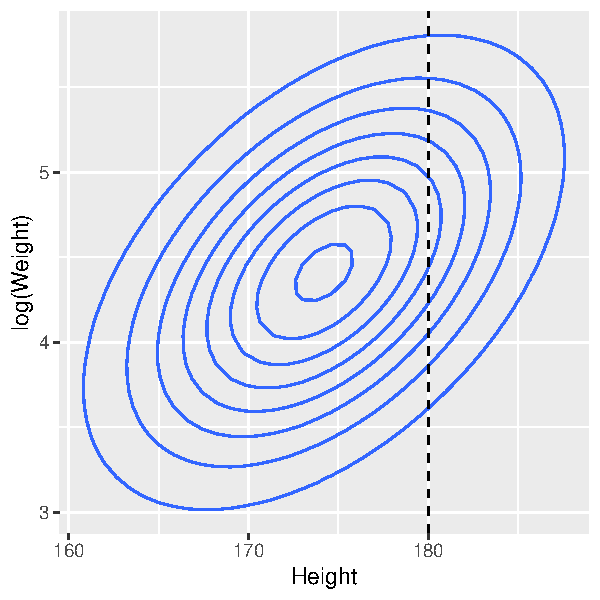
\includegraphics[height=.7\textheight]{figure/example-25-3-1}
    \end{center}
  \end{block}
\end{frame}

\begin{frame}
  \begin{block}{\examplectd}
    \begin{enumerate}[a)]
      
    \item What is the joint pdf of $X$ and $Y$? 

    \item Are height and the log of weight independent?
      
    \item What is the marginal distribution of height?
      
    \item What is the conditional distribution of the log of weight for a man 180~cm tall? 
    
    \item Is it unusual for a 180~cm tall man to weigh 70~kg?
    \end{enumerate}
  \end{block}
\end{frame}

\begin{frame}
  \frametitle{\invisible{Hello}}
  
  \begin{center}
    \Large{\textbf{5.3 Conditional Distributions}}

    \bigskip

    \Large{Mean and Variance via\\ the Conditional Mean and Variance}
  \end{center}
  
\end{frame}

\begin{frame}

  \begin{block}{Conditional Mean and Variance Formulas}
  For any two random variables, $X$ and $Y$,
  \begin{align*}
      E(Y)&=E[E(Y|X)]\\
      V(Y)&=E[V(Y|X)] + V[E(Y|X)].
  \end{align*}
    \end{block}
\end{frame}

\begin{frame}

  \begin{block}{Conditional Mean and Variance Formulas}
  More explicitly, for any two random variables, $X$ and $Y$,
  \begin{align*}
      E(Y)&=E_{X}[E_{Y|X}(Y|X)]\\
      V(Y)&=E_{X}[V_{Y|X}(Y|X)] + V_X[E_{Y|X}(Y|X)].
  \end{align*}
    \end{block}
\end{frame}

\begin{frame}
  \begin{block}{\examplectd}
    \begin{enumerate}[a)]
      
    \item What is the joint pdf of $X$ and $Y$? 

    \item Are height and the log of weight independent?
      
    \item What is the marginal distributions of height?
      
    \item What is the conditional distribution of the log of weight for a man 180~cm tall? 
    
    \item Is it unusual for a 180~cm tall man to weigh 70~kg?

    \item Verify the formulas for computing the mean and variance of $Y$ from the conditional mean and variance formulas for the case of two bivariate normal random variables. 
      
    \end{enumerate}
  \end{block}
\end{frame}

\begin{frame}<handout:0>
  \begin{center}
    \Huge{\textbf{Questions?}}
  \end{center}
\end{frame}

\begin{frame}

\begin{block}
The daytime mean temperature for London in November is approximately normally distributed with a mean of 3.4~C and standard deviation of 1.7~C. Suppose that the joint distribution of the temperature subsequent days is bivariate normal with a correlation of $.6$. 

Let $T_1$ and $T_2$ be the temperature on two different days.

\begin{enumerate}
\item Sketch a plot showing contours of the joint pdf of $T_1$ and $T_2$. 
\item What is the distribution of $T_2$ given $T_1=1$~C? Be as specific as possible.
\item Explain the result in terms of the phenomenon of regression to the mean. 
\end{enumerate}
\end{block}

\end{frame}
\end{document}
